\documentclass[conference]{IEEEtran}
\IEEEoverridecommandlockouts
\usepackage{cite}
\usepackage{amsmath,amssymb,amsfonts}
\usepackage{algorithmic}
\usepackage{graphicx}
\usepackage{textcomp}
\usepackage{xcolor}
\usepackage{hyperref}
\usepackage{placeins}
\usepackage[spanish, mexico]{babel}
\def\BibTeX{{\rm B\kern-.05em{\sc i\kern-.025em b}\kern-.08em
    T\kern-.1667em\lower.7ex\hbox{E}\kern-.125emX}}
\usepackage[table,xcdraw]{xcolor}

\title{Análisis de Sentimiento con Reseñas de IMDB}

\author{\IEEEauthorblockN{
Dora Alicia Guevara Villalpando \\
Matrícula: 1551003}
\\
\IEEEauthorblockA{\textit{Universidad Autónoma de Nuevo León)} \\
\textit{Facultad de Ciencias Físico Matemáticas}\\
Maestría en Ciencia de Datos \\
Procesamiento y Clasificación de Datos\\\\
dora.guevaravll@uanl.edu.mx}
}

\date{\today}

\begin{document}

\maketitle


\section{Introducción}

El análisis de sentimiento es una tarea fundamental en el campo de la minería de texto y el aprendizaje automático. Este tipo de análisis permite identificar las emociones o actitudes expresadas en textos, como positivas, negativas o neutrales. En el contexto de las reseñas de usuarios, es especialmente útil para comprender la percepción del público hacia productos, servicios o contenidos.

En este proyecto, se empleó el conjunto de datos \textit{IMDB Movie Reviews}, que contiene 50,000 reseñas de películas etiquetadas como positivas o negativas. Este dataset es ampliamente utilizado en la comunidad de aprendizaje automático debido a su balance entre clases y la complejidad del lenguaje natural empleado en las reseñas.

El objetivo principal fue desarrollar un modelo capaz de predecir el sentimiento de las reseñas con un alto grado de precisión. Para lograr esto, se exploraron técnicas clásicas de representación de texto y clasificación, evaluando tres enfoques: \textit{Logistic Regression}, \textit{Support Vector Machines (SVM)} y \textit{Random Forest}. Este trabajo también buscó comparar el rendimiento de los modelos para recomendar el más adecuado según las características del dataset y las necesidades del análisis.

\section{Metodología}

\subsection{Selección del Dataset}

El dataset utilizado, \textit{"IMDB Movie Reviews"}, fue descargado desde el repositorio de Stanford. Este conjunto de datos está dividido equitativamente en dos subconjuntos: 25,000 reseñas para entrenamiento y 25,000 reseñas para prueba. Cada reseña tiene una etiqueta binaria que indica si el sentimiento es positivo o negativo. La estructura del dataset permitió realizar una división adicional del conjunto de entrenamiento en datos de validación para ajustar los modelos.


\subsection{Preprocesamiento}

El preprocesamiento de los datos incluyó:

\begin{enumerate}
    \item Limpieza del texto: Se eliminaron etiquetas HTML, caracteres no alfanuméricos y espacios extra.
    
    \item Normalización: Las reseñas se convirtieron a minúsculas para garantizar consistencia.
    
    \item Eliminación de stop words: Durante la vectorización, se excluyeron palabras comunes que no aportan información significativa al análisis (como "the", "and", etc.).
\end{enumerate}


\subsection{Vectorización}

Para transformar las reseñas en un formato numérico adecuado para los modelos de clasificación, se utilizó el método \textbf{TF-IDF (Term Frequency-Inverse Document Frequency)}. Esta técnica mide la importancia de una palabra dentro de un documento en relación con el corpus completo. Se seleccionó un máximo de 5000 características, lo que permitió capturar las palabras más relevantes sin sobrecargar el modelo con dimensionalidad excesiva.


\subsection{Modelos Evaluados}

\begin{itemize}
    \item \textbf{Logistic Regression:} Este modelo lineal es eficiente y altamente interpretable. Es adecuado para tareas donde las características tienen una relación lineal con las etiquetas de salida.
    
    \item \textbf{Support Vector Machines (SVM):} Utilizando un kernel lineal, este modelo busca maximizar los márgenes entre clases en espacios de alta dimensión, como los generados por TF-IDF.
    
    \item \textbf{Random Forest:} Este enfoque basado en conjuntos utiliza múltiples árboles de decisión para capturar patrones no lineales y manejar datos complejos.
\end{itemize}

Cada modelo fue entrenado utilizando el conjunto de datos de entrenamiento y evaluado en el conjunto de validación. Las métricas clave, como precisión, recall, F1-score y exactitud, fueron utilizadas para comparar su desempeño.



\section{Resultados}

\subsection*{Logistic Regression}
\begin{itemize}
\item \textbf{Precisión}: 0.89 (clase negativa), 0.86 (clase positiva).
\item \textbf{Recall}: 0.86 (clase negativa), 0.89 (clase positiva).
\item \textbf{F1-Score}: 0.87-0.88.
\item \textbf{Exactitud Global}: 0.87.
\end{itemize}

\subsection*{Support Vector Machines (SVM)}
\begin{itemize}
\item \textbf{Precisión}: 0.88 (clase negativa), 0.86 (clase positiva).
\item \textbf{Recall}: 0.86 (clase negativa), 0.89 (clase positiva).
\item \textbf{F1-Score}: 0.87.
\item \textbf{Exactitud Global}: 0.87.
\end{itemize}

\subsection*{Random Forest}
\begin{itemize}
\item \textbf{Precisión}: 0.83 (clase negativa), 0.85 (clase positiva).
\item \textbf{Recall}: 0.85 (clase negativa), 0.83 (clase positiva).
\item \textbf{F1-Score}: 0.84.
\item \textbf{Exactitud Global}: 0.84.
\end{itemize}


\section{Análisis comparativo}

Acorde a lo que se observa en la tabla \ref{tab:comparación}:

\begin{table}[h!]
    \centering
    \begin{tabular}{| l | c | c |}
    \rowcolor[HTML]{FFCCC9} 
    \hline
        \multicolumn{1}{c}{\cellcolor[HTML]{FFCCC9}\textbf{Modelo}} & \textbf{Exactitud} & \textbf{F1 Score Promedio} \\ \hline
        Logistic Regression & 0.87 & 0.87 \\
        SVM & 0.87 & 0.87 \\
        Random Forest & 0.84 & 0.84 \\ \hline
    \end{tabular}
    \caption{Análisis comparativo}
    \label{tab:comparación}
\end{table}

\FloatBarrier

\begin{enumerate}
    \item \textbf{Logistic Regression} y \textbf{SVM} mostraron desempeños casi idénticos, con una exactitud del 87\% y F1-Score promedio de 0.87.
     
    \item \textbf{Random Forest} tuvo un desempeño inferior con una exactitud del 84\%, lo que sugiere que no es tan efectivo en este tipo de representación vectorial (TF-IDF).
\end{enumerate}

Para el primer libro se obtuvo la siguiente nube de palabras:

\begin{figure}[h]
    \centering
    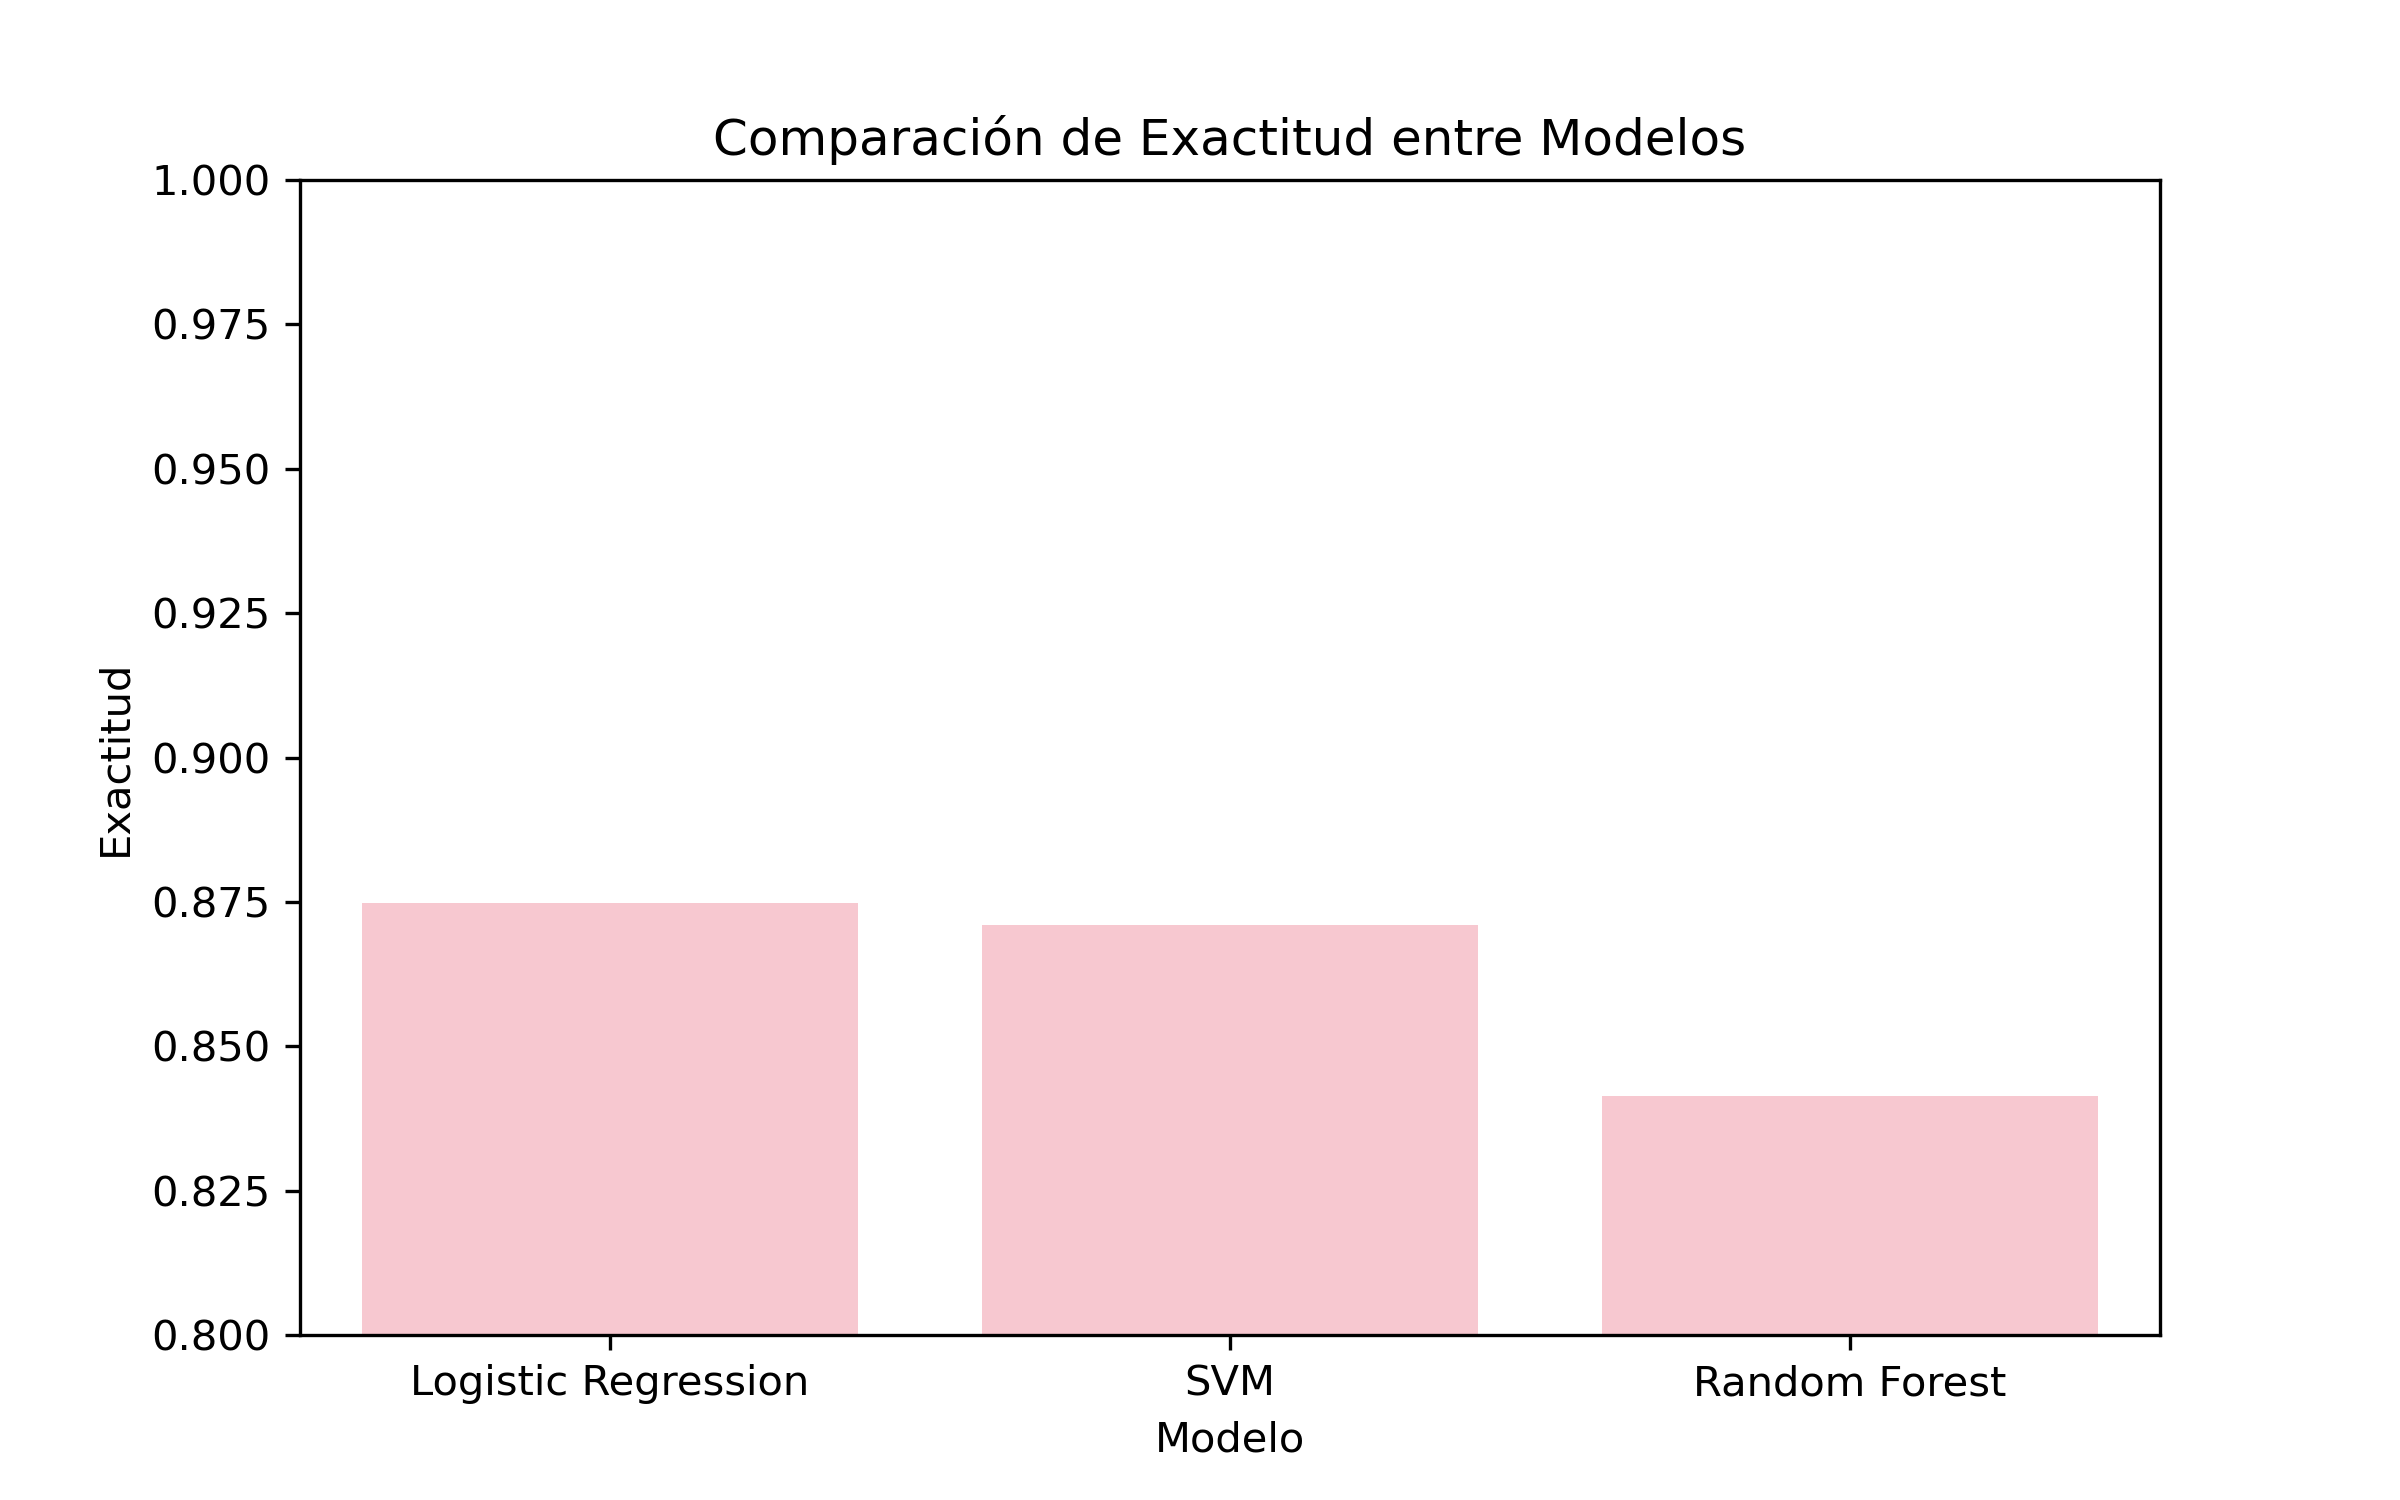
\includegraphics[width=0.8\linewidth]{Comparacion_Modelos.png}
    \caption{Comparación.}
    \label{fig:comp}
\end{figure}

\FloatBarrier


\section{Conclusiones}

\begin{enumerate}
    \item \textbf{Modelo Recomendado}:
    \begin{itemize}
        \item \textbf{Logistic Regression} es la mejor opción si se prioriza simplicidad y velocidad.
        \item \textbf{SVM} es una alternativa igualmente válida si se busca robustez en otras configuraciones.
    \end{itemize}
    
    \item \textbf{Modelo Descartado}:
    \begin{itemize}
        \item \textbf{Random Forest}, aunque flexible, no fue competitivo en este escenario.
    \end{itemize}
    
    \item \textbf{Futuras Mejoras}:
    \begin{itemize}
        \item Probar modelos basados en \textit{embeddings} preentrenados como BERT para mejorar el desempeño.
        \item Incrementar el conjunto de datos para explorar el impacto en modelos más complejos.
    \end{itemize}
\end{enumerate}


\section*{Referencias}

\begin{itemize}
    \item Dataset: IMDB Movie Reviews (\url{https://ai.stanford.edu/~amaas/data/sentiment/})

    \item Métodos: Scikit-learn Library (TF-IDF, Logistic Regression, SVM, Random Forest)

    \item Análisis de texto (text mining) con Python. (\url{https://cienciadedatos.net/documentos/py25-text-mining-python}) 
\end{itemize}


\end{document}